\chapter{Related Work}

Nowadays, many scholars worldwide have submitted research projects relating to turning sign language into text, using a variety of methodologies and perspectives.

Two main approaches have been proposed:
\begin{itemize}
  \item \textbf{Glove-based approaches:} This approach requires the deaf and mute to wear a sensor glove. When users have any different actions or gestures, the gloves will record all those movements. After that, data from the sensor will be analyzed by the analyzer component. Finally, that component returns the output to the users.
  \item \textbf{Vision-based approaches:} With this approach, developers will apply image processing algorithms to determine hand positions, gestures, and movements. The user will not have to wear necessary glove-based methods, which is convenient. However, using image processing algorithms, we need to deal with the worst quality output affected by these algorithms.
\end{itemize}

Specifically, about the vision-based approach, the earlier method used several image processing algorithms to build feature vectors based on a single RGB image of the hand. In this paper, "Real-time sign language recognition using a consumer depth camera" \cite{kuznetsova2013real}, using multi-layered random forest (MLRF) not only allows them to recognize hand signs correctly but also minimizes training time and effort. Alternatively, in this paper, "Sign Language Translation in Urdu/Hindi Through Microsoft Kinect," sign language can be recognized by auxiliary equipment: Microsoft Kinect (see Figure \ref{fig:Chap2-MS-Kinect}), which captures the signs of the deaf person, after that, through the computer system, they can detect what deaf people say.

\begin{figure}[H]
  \centering
  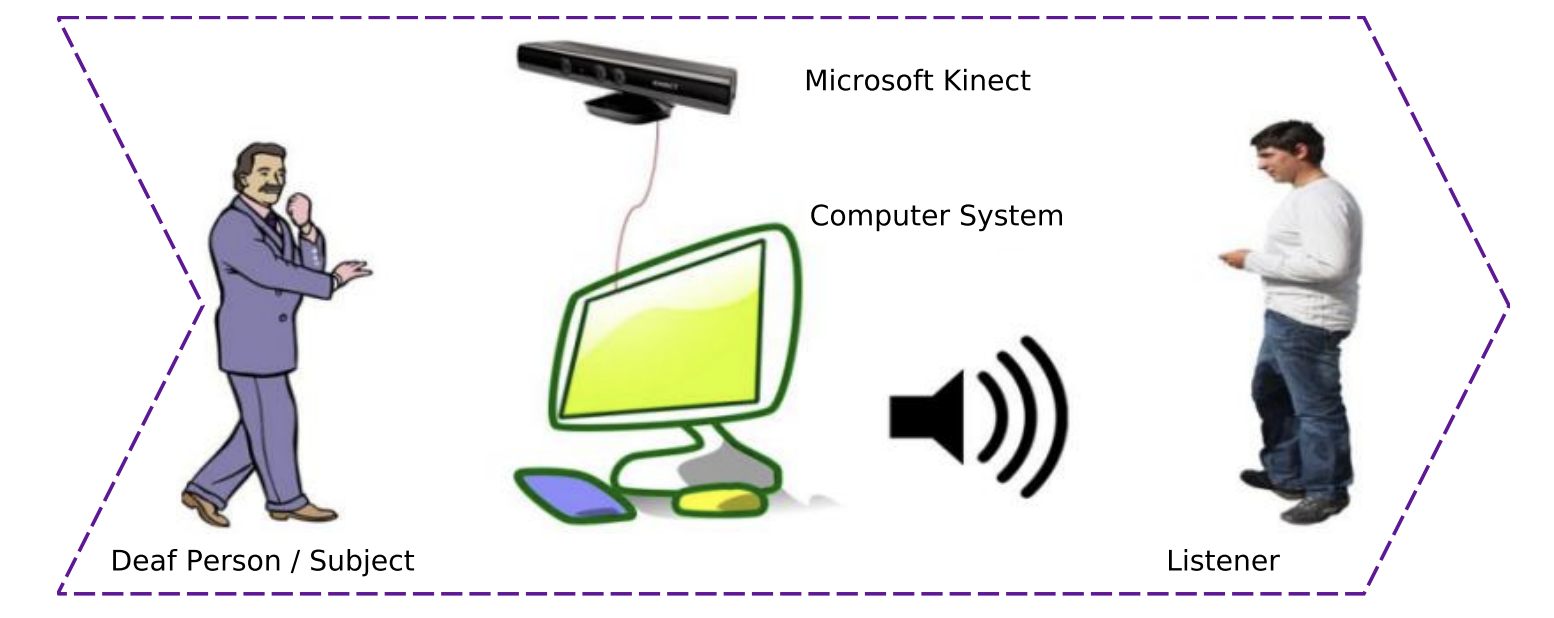
\includegraphics[width=\textwidth]{img/Chap2/MS-Kinect.png}
  \caption{Using Microsoft Kinect to translate sign language}
  \label{fig:Chap2-MS-Kinect}
\end{figure}

Besides the vision-based approach, glove-based system has a much relevant research. This paper, "The Language of Glove: Wireless gesture decoder with low-power and stretchable hybrid electronics" \cite{o2017language} introduces the way to convert American Sign Language (ASL) alphabet into text and display it on a computer or smartphone (see Figure \ref{fig:Chap2-Glove-Base}). They can detect which hand gesture is performed with sensor gloves and send the result to the smartphone via Bluetooth. The sign language interprets text and displays it on the digital display screen. This approach is helpful in the real world for the deaf and mute who cannot communicate with ordinary people.

\begin{figure}[H]
  \centering
  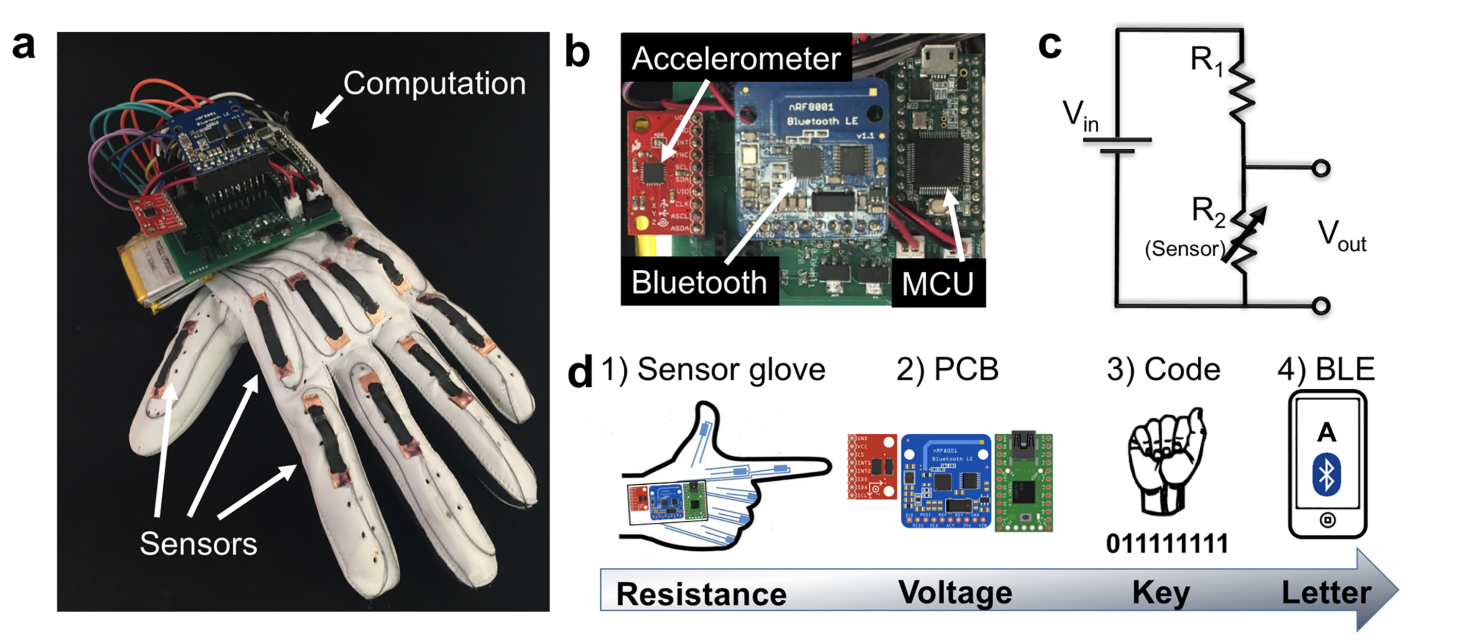
\includegraphics[width=\textwidth]{img/Chap2/Glove-Based.png}
  \caption{Glove-based approach to translate sign language}
  \label{fig:Chap2-Glove-Base}
\end{figure}

Both approaches above have some problems; they can only recognize a minimal number of words, like an alphabet, number, or some word with easy hand shape and no motion. However, it is not easy; many words will use the same hand shape but differ in many characteristics, such as positions and directions. There is currently no model that can handle the conversion of sign language flexibly and conveniently for the deaf and mute, helping them communicate effectively and naturally. Therefore, thanks to applying appropriate technologies, the authors carry out this graduation thesis to break down the barriers between deaf-and-mute people and ordinary people, helping them become self-sufficient and more confident in daily communication.

